\section{Theoretische Grundlagen}

In diesem Kapitel werden die grundlegenden Begriffe und Konzepte erläutert, welche wichtig für das Verständnis der Arbeit sind. Es wird zunächst der DevOps-Ansatz und das Architekturmuster der Microservices beschrieben. Anschließend wird Containervirtualisierung sowie Kubernetes erklärt.

\subsection{DevOps}

Alle der in diesem Kapitel beschriebenen Architekturmuster, Methoden und Werkzeuge lassen sich dem DevOps-Ansatz zuordnen. Für das Verständnis der Arbeit ist es also essentiell zu Verstehen was DevOps bedeutet und warum es so populär ist. Wie das Kofferwort "DevOps" bereits andeutet, beschreibt er einen Ansatz für eine effektivere und stärkere Zusammenarbeit zwischen Softwareentwicklung (Development) und IT-Betrieb (Operations). Für DevOps gibt es keine einheitliche Definition. Es ist ein Überbegriff für Denkweisen, Kultur, Methoden, Technologien und Werkzeuge. Der Kundennutzen wird dabei immer in den Mittelpunkt gestellt [\cite[S. 1]{halstenbergDevOps2020}]. Das Ziel ist es die Softwarequalität zu verbessern und die Geschwindigkeit der Entwicklung und Bereitstellung zu erhöhen [\cite[S. 6]{arundelCloud2019}]. Um die Ziele umzusetzen bedient sich DevOps etablierten Methoden und Werkzeuge um daraus einen ganzheitlichen Ansatz zu formulieren. \\
\\
DevOps wird immer wichtiger, da durch das Aufkommen von Cloud Computing die Entwicklung und der Betrieb von Anwendungen nicht mehr trennbar ist. DevOps in ein Unternehmen einzuführen ist ein langwieriger Prozess, da insbesondere die Unternehmenskultur transformiert werden muss. Vor allem in großen Unternehmen zeigt sich das viele Prozesse schwerfällig geworden sind und nicht mehr dem eigentlichen Kundennutzen dienen. DevOps soll dieses Problem lösen und Unternehmen wieder anpassungsfähiger machen, ohne geordnete Strukturen zu verlieren.

\begin{figure}[H] 
    \centering
    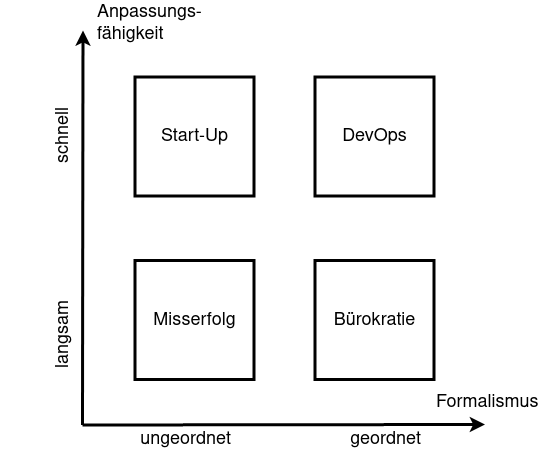
\includegraphics[width=0.6\textwidth]{figures/DevOpsDiagramm.png}
    \caption{Kategorisierung von Unternehmen [\cite[S. 11]{halstenbergDevOps2020}]}
\end{figure}

Eine reduzierte Time-to-Market kann durch engere Abstimmung und Automatisierung erreicht werden. Die Time-to-Market gibt an, wie lange es dauert eine Änderung zum Kunden, also auf die Produktionsumgebung, zu bringen. So können Änderungen schnell ausgeliefert werden und Feedback vom Endanwender erreicht schneller die Entwickler. Zur Umsetzung können Methoden wie Continuous-Integration und Continuous-Delivery eingesetzt werden, aber auch Architekturmuster wie Microservices und Werkzeuge wie Docker und Kubernetes können dabei unterstützen.

\subsection{Microservices}

Im Mittelpunkt dieser Arbeit stehen Microservices. Bei Microservices handelt es sich um ein Architekturmuster zur Modularisierung von Software (\cite[S. 15]{newmanMicroservices2015}). Eine einheitliche Definition für Microservices gib es nicht [\cite[S. 2]{wolffMicroservices2018}]. Bei der Beschreibung von Microservices werden grundlegende Prinzipien einer standardisierten Definition vorgezogen.

\subsubsection{Merkmale}

Microservices sind das Gegenteil von klassischen monolithischen Softwarearchitekturen. Ein Monolith ist eine einzelne, zusammenhängende und untrennbare Einheit. Die Erweiterbarkeit und Wartbarkeit von Monolithen ist häufig komplex, da die Codebasis umfangreich ist und mit der Zeit immer stärker wächst. Die Arbeit von mehreren Entwicklerteams ist ineffizient, dar ein höher Abstimmungsbedarf nötig ist. Des Weiteren lässt ist die Skalierbarkeit des schwergewichtigen Monolithen sehr beschränkt. Durch Modularisierung einer Anwendung lassen sich diese Probleme abschwächen, können jedoch nicht komplett behoben werden.

\begin{figure}[H] 
    \centering
    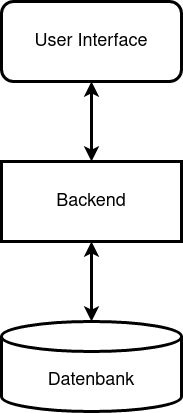
\includegraphics[width=0.2\textwidth]{figures/Monolith.png}
    \caption{Beispielhafter Aufbau einer monolithischen Architektur}
\end{figure}

Genau hier setzten Microservices an. Obwohl der Begriff Microservices noch realtiv jung ist, sind die dahinterstehenden Konzepte bereits deutlich älter [\cite[S. 15]{newmanMicroservices2015}]. Zur Verständlichkeit und leichteren Weiterentwicklung werden große Systeme werden schon lange in kleine Module unterteilt. Die Besonderheit von Microservices liegt darin, dass die Module einzelne Programme sind. Das Architekturmuster der Microservices zählt zu den verteilten Systemen. Die einzelnen Microservices laufen zumeist auf vielen unterschiedlichen Rechnern und kommunizieren über das Netzwerk.

\begin{figure}[H] 
    \centering
    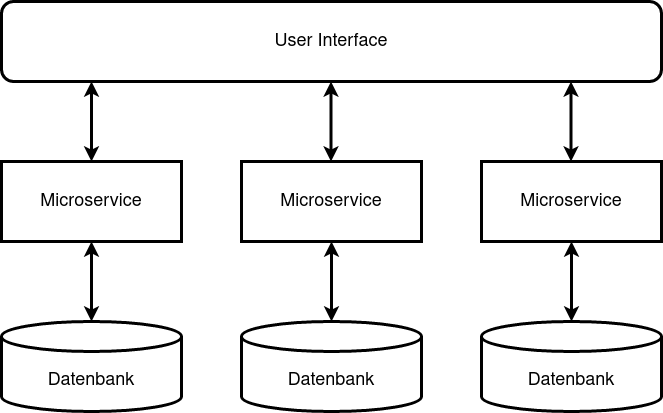
\includegraphics[width=0.71\textwidth]{figures/Microservices.png}
    \caption{Beispielhafter Aufbau einer Microservice-Architektur}
\end{figure}

Ein einzelner Microservice soll eine Aufgabe bestmöglich erledigen. Dieser Ansatz ist angelehnt an die \acs{UNIX}-Philosophie: "Mache nur eine Sache und mache sie gut" [\cite[]{salusQuarter1994}]. Jeder Microservice bildet so eine klar definierte Funktion des Gesamtsystems ab. Die Microservices müssen eigenständig sein, sodass sie unabhängig voneinander verändert und bereitgestellt werde können. Die Kommunikation zwischen den Microservices erfolgt ausschließlich über das Netzwerk mittels sprachunabhängiger Schnittstellen, sogenannte \acp{API} [\cite[S. 64]{trempArchitekturen2021}]. \\
\\
Die Größe eines Microservices ist nicht zwangsläufig entscheidend [\cite[S. 2]{wolffMicroservices2018}]. Der Name "Microservices" deutet bereits an, dass es sich um kleine Services handelt, jedoch ist eine genaue Festlegung der Größe nicht sinnig [\cite[S. 22]{newmanMicroservices2015}]. Eine Messung der Größe durch die Anzahl der Codezeilen wäre zwar denkbar, jedoch hängen derartige Kriterien stark von der verwendeten Programmiersprache ab. Stattdessen sollte sich die Größe an fachliche Gegebenheiten anpassen. Je kleiner die Services gestaltet werden, umso stärker kommen die in den nachfolgenden Abschnitten beschriebenen Vor- und Nachteile zur Geltung. Eine Obergrenze für die Größe eines Microservices stellt die Teamgröße dar. An einem Microservice darf immer nur ein Entwicklerteam arbeiten [\cite[S. 23]{newmanMicroservices2015}]. Kann der Microservice nicht mehr von einem Team alleine entwickelt und gewartet werden, so ist er zu groß. Ein Microservice sollte auch nur so groß sein, dass er von einem Entwickler allumfassend verstanden werden kann. Ein Microservice sollte jedoch auch nicht zu klein gewählt werden, da ansonsten der Aufwand für die Bereitstellung der vielen Microservices sehr groß wird und die Kommunikation über das Netzwerk ansteigt. \\
\\
Um von Microservices zu profitieren müssen Strukturen in Unternehmen überarbeitet werden. Das Gesetz von Conway besagt, dass durch die Kommunikationsstrukturen einer Organisation auch die Struktur der Systeme, welche die Organisation entwirft, vorgegeben wird [\cite{conwayHow1968}]. Bei monolithischen Anwendungen werden die Entwicklerteams häufig nach ihrem Fachbereich aufgeteilt. Es bilden sich so beispielsweise Teams spezialisiert auf das Frontend, das Backend und die Datenbank. Die entwickelte Anwendung wird, nach dem Gesetz von Conway, auch aus diesen drei Bereichen bestehen. Wenn nun ein neues Feature umgesetzt werden soll, müssen sich alle drei Teams miteinander absprechen. Um eine Microservice-Architektur umzusetzen muss also auch die Struktur des Unternehmens verändert werden. Die Entwicklerteams müssen crossfunktional mit Spezialisten aus verschiedenen Fachbereichen aufgebaut werden. Der Vorteil ist das Änderungen so häufig nur ein Entwicklerteam betreffen und der Koordinationsaufwand sinkt. \\
\\
Microservices werden häufig mit \ac{SOA} in Verbindung gebracht. Microservices übernehmen viele Prinzipien von \ac{SOA}. \ac{SOA} ist ein Ansatz mit dem Ziel Funktionalitäten von betrieblichen Anwendungen durch Services von außerhalb zugreifbar zu machen [\cite[S. 2]{wolffMicroservices2018}]. Ein Service bildet in diesem Kontext einen Geschäftsprozess ab. Dadurch soll Flexibilität und Wiederverwendbarkeit in der IT von Unternehmen erhöht werden. Es gibt also durchaus viele Parallelen zu Microservices, jedoch setzen sie an verschiedenen Ebenen an. Während Microservices ein konkretes Architekturmuster für ein einzelnes System ist, beschreibt \ac{SOA} wie viele Systeme in einem Unternehmens miteinander interagieren können. \\
\\

\subsubsection{Vorteile}

Bei monolithischen Anwendungen, entstehen schnell unerwünschte Abhängigkeiten zwischen verschiedenen Komponenten. Die vielen Abhängigkeiten sind schwer zu überblicken und die Änderung von einer Komponente wird erschwert, da es zu unerwünschten Nebeneffekten kommen kann. In der Praxis wird so die Architektur von den Monolithen mit der Zeit zunehmend schlechter [\cite[S. 3]{wolffMicroservices2018}]. Die Microservices besitzen nur eine lose Kopplung über explizite Schnittstellen. Unerwünschte Abhängigkeiten treten dadurch seltener auf. Durch die expliziten Schnittstellen ist es auch einfach einen gesamten Microservice zu ersetzten. Der neue Microservice muss lediglich die selbe Schnittstelle anbieten wie der Alte. Das neu schreiben eines Microservices ist durch die begrenzte Größe in der Regel nicht schwer. Somit können Microservices schneller zu neuen Technologie-Stacks migriert werden. Die Ablösung von großen Monolithen gestaltet sich dagegen häufig als eine fast unmögliche Aufgaben [\cite[S. 29]{newmanMicroservices2015}]. 

Microservices können auch unabhängig voneinander skaliert werden. So kann eine einzelne Funktionalität, welcher stärker genutzt wird, einzeln hoch skaliert werden, ohne das gesamte System zu skalieren [\cite[S. 5]{wolffMicroservices2018}]. Flaschenhälse welche eine Anwendung ausbremsen, können somit besser vermieden werden. Die Last kann durch Microservices auch besser verteilt werden, da sie auf unterschiedlichen Rechnern laufen können. Durch Microservices können so Kosten eingespart werden. Es gibt wenige Architekturmuster wie dieses, welche so eng mit Kosteneinsparungen verbunden sind. (\cite[S. 27]{newmanMicroservices2015}).

Die Unabhängigkeit der Microservices führt zu einer großen Technologiefreiheit. Die eingesetzten Technologien müssen lediglich die entsprechende Schnittstelle anbieten können [\cite[S. 5]{wolffMicroservices2018}]. Somit kann für jeden Microservice kompromisslos die am besten geeignete Technologie gewählt werden. Dadurch sinken auch die möglichen Auswirkungen von falschen Entscheidungen bei der Technologieauswahl.

Ein weiterer wesentlicher Grund für Microservices ist \ac{CD}. Die Microservices können unabhängig voneinander bereitgestellt werden. Tritt bei einer Bereitstellung ein Fehler auf, sind die verbundenen Risiken deutlich geringer. Es ist nicht das gesamte System davon betroffen, sondern nur der entsprechende Service. Dadurch, dass nur der veränderte Microservice neu bereitgestellt werden muss, ist die Bereitstellung schneller als bei einem Monolithen. Vor allem bei geringen Änderungen ist die erneute Bereitstellung eines gesamten Monolithen sehr unliebsam. Außerdem kann zur Absicherung bei Microservices leicht parallel eine alte Version des Microservices betrieben werden. Bei Monolithen wäre in so einem Fall der Ressourcenverbrauch doppelt so hoch, wie die Anwendung eigentlich benötigt.

\subsubsection{Herausforderungen}

Doch natürlich haben Microservices wie jedes Architekturmuster auch einige Nachteile. Die Aufteilung eines Systems in viele Microservices erhöht die Komplexität. 

Die Beziehungen unter den Microservices können schnell unüberschaubar werden. Welcher Microservice eine Schnittstelle eines anderen Microservices benutzt oder benötigt kann von außen nicht direkt eingesehen werden. Dies ist aber wichtig, um zu Wissen, welche Microservices von der Änderung einer Schnittstelle betroffen werden. Auch muss dabei geachtet werden, dass es auf Code-Ebene nicht zu ungewollten Abhängigkeiten kommt. Wenn mehrere Microservices die selbe Bibliothek verwenden, geht die Unabhängigkeit verloren und die Microservices müssen unter umständen gemeinsam bereitgestellt werden [\cite[S. 75]{wolffMicroservices2018}].

Bei Monolithen können Teile des Codes leicht von einer Komponente in eine Andere verschoben werden kann. Bei Microservices müssen die Teile in einen anderes eigenständiges Programm verschoben werden und der Aufwand ist deutlich höher. Die Auswirkungen von Fehlentscheidungen bei der Einteilung und Abgrenzung sind somit sehr hoch, weil ein Refactoring über mehrere Microservices kompliziert ist.

Microservices sind verteilte Systeme und bringen auch die damit verbundenen Nachteile mit sich. Da die Kommunikation mit den Microservices über das Netzwerk läuft, ist die Antwortzeit der Microservices von der Latenz abhängig. Da wird vor allem dann problematisch wenn ein Microservice viele Dienste von anderen Microservices in Anspruch nimmt. Deshalb sollten Microservices untereinander möglichst wenig kommunizieren müssen. Besitzen zwei Microservices viele Abhängigkeiten, kann dies ein Hinweis auf eine falsche Einteilung der Microservices sein. Des Weiteren muss das Netzwerk die höhere Last durch die Aufrufe standhalten. Außerdem ist Kommunikation über das Netzwerk immer unzuverlässig.

Die technologische Freiheit der Microservices kann schnell zu einer Herausforderung werden. Wenn jeder Microservice einen komplett unterschiedlichen Technologie-Stack verwendet, steigt die Komplexität des Gesamtsystems. Auch wird der Wechsel von Mitarbeitern zu anderen Teams schwieriger. Es bietet sich also an den Technologie-Stack einzuschränken und übergreifende Richtlinien für alle Microservices zu bestimmen.

Der Betrieb von Microservices ist sehr komplex. Die vielen Microservices müssen orchestriet werden.

\subsubsection{Architektur}

Die Architektur bei Micrservices ist das Finden von Kompromissen. Die einzelnen Entwicklerteams sollten viel Freiheit haben, um die nach ihrer Meinung am Besten geeigneten Technologien für ihren Service zu verwenden. Es macht jedoch Sinn gewisse Vorgaben und Rahmenbedingungen vorzugeben. Die Beschränkung auf eine Auswahl von beispielsweise fünf Programmiersprachen macht Sinn, um Wissen nicht zu weit zu verstreuen. Für die Schnittstellen ist es sinnvoll einige wenige Schnittstellenarten festzulegen, die von allen Services verwendet wird.  \\
\\
Die Mikroarchitektur, also die Architektur mit der ein einzelner Service implementiert wurde, sollte von außen nicht sichtbar sein und besitzt somit für das Gesamtsystem keine Relevanz. \\
\\
Die fachliche Archtiektur, also die Aufteilung in verschiedene Bereiche, die jeweils von einem Microservice umgesetzt werden. Wo bei dieser Aufteilung die Grenzen gezogen werden ist eine der zentralen Herausforderungen (\cite[S. 102]{wolffMicroservices2018}). Das entscheidende Kriterium für die Aufteilung ist, dass Änderungen möglichst nur einen Service betreffen und somit von nur einem Team durchgeführt werden können. Dadurch ist wenig Abstimmung zwischen den Entwicklerteams notwendig und die Vorteile der Microservices kommen erst richtig zur geltung. Jeder Microservice solle also eine fachlichen Kontext darstellen, der eine abgeschlossene Funktionalität darstellt. \\
\\
Natürlich sind die Microservices nie vollständig voneinander unabhängig. Es wird Services geben die, die Funktionalität anderer Services aufrufen. Zu viele solcher Verbindungen führen jedoch zu einer hohen Abhängigkeit und widersprechen dem Microservice-Ansatz. Eine lose Kopplung, also nur wenige Abhängigkeiten sind erstrebenswert, da so sich Änderungen so nur auf einen Service auswirken. Benötigt ein Microservice viele Funktionalitäten von einem anderen Microservice kann das ein Hinweis auf eine schlechte Aufteilung sein und die Services sollten an einer anderen Stelle aufgeteilt werden oder womöglich direkt zusammen gelegt werden. Innerhalb eines Micrservice sollten die Komponenten und Module des Programms jedoch eine starke Kopplung besitzen. Dadurch wird gewährleistet, dass die Bestandteile wirklich zusammengehören. \\
\\
Zyklische Abhängigkeiten sind auch zu vermeiden, da dort ohne weitere Abstimmung Änderungen in einem der beiden Services nicht möglich sind. \\
\\
Eine bewährter Ansatz für den Anfang der Architektur ist es, mit großen Service zu beginnen und diese aufzuteilen. Einen großen Service aufzuteilen ist einfach. Die Gesamtarchitektur von vielen kleinen Services zu überarbeiten jedoch sehr komplex. \\

Herausforderung: Microservice-Systeme sind schwer änderbar (auf Makro Ebene)

Architektur eines Microservice: Erklärung Schichtenarchitektur, wenige Vorgaben, wird vom Team gehandhabt

Für die Skalierbarkeit ist es wichtig, dass mehrere Instanzen vom selben Microservice gestartet werden können. Das bedeutet, dass Microservices keinen Zustand speichern dürfen.
Es ist ratsam, dass jeder Microservice eine eigene Datenbank besitzt. Das führt zu einer dezentralen Datenbankstruktur im System. Dadurch sind die Datenschemata weniger komplex und genau auf die Anforderungen des einen Microservices spezialisiert.  Wenn Datenbanken von mehreren Microservices verwendet werden ist bei Änderungen an der Datenbank ein höher Abstimmungsaufwand nötig.

Die lose gekoppelten Microservices dürfen keinen Zustand speichern. Nur so können mehrere Instanzen vom selben Microservice gestartet werden und die 

\subsubsection{Integration}

Microservices müssen miteinander kommunizieren. Die Integration der Services ist auf drei verschiedenen Ebenen denkbar.

\paragraph{UI}

\paragraph{Datenbank}

\paragraph{Microservices}

Zuletzt müssen natürlich auch Microservices direkt miteinander kommunizieren, um so Funktionalität von anderen Services aufzurufen. Die meist verbreitetste Technologie ist HTTP REST. Es gibt auch weitere Ansätze wie SOAP oder Message-Systeme.

Als Application Programming Interface (API) wird eine Programmierschnittstelle bezeichnet. Diese Schnittstellenart, erlaubt anderen Programmen die Anbindung an ein System. Bei der Schnittstelle, die in diesem Projekt entworfen wird, handelt es sich um eine sogenannte Programmierschnittstelle. Mit einer API wird sichergestellt, dass die Unternehmensinfrastruktur flexibel, zukunftssicher und nicht abhängig von einer einzigen Technologie bleibt. Auch können mit einer API ganz einfach Daten freigegeben und universell zur Verfügung gestellt werden. [\cite[S. 95ff]{koflerDigitale2018}]

Die API in diesem Projekt soll nach dem REST-Architekturstil erstellt werden. Representational State Transfer (REST) ist ein weit verbreitetes Paradigma, welches die Struktur und das Verhalten von Schnittstellen vereinheitlichen soll. Eine REST-API verwendet HTTP-Anfragen mit verschiedenen HTTP-Anfragemethoden, um auf Daten zuzugreifen. Jeder Endpunkt einer REST-API muss eine eindeutige Adresse, den Uniform Resource Locator (URL), besitzen. [\cite[S. 76ff]{fieldingArchitectural2000}]

REST basiert auf den folgenden sechs Prinzipien:
\begin{itemize}
\item Client-Server: Ein Server stellt einen Dienst bereit, der bei Bedarf vom Client angefragt wird.
\item Zustandslosigkeit: Jede Anfrage eines Clients ist in sich geschlossen und enthält alle benötigten Informationen.
\item Caching: HTTP-Caching soll verwendet werden.
\item Einheitliche Schnittstelle: Die Ressourcen sollen klar adressierbar sein und alle Nachrichten sollen selbstbeschreibend sein.
\item Mehrschichtige Systeme: Die Systeme sollen mehrschichtig aufgebaut sein.
\item Code on Demand: Nur im Bedarfsfall wird Code an den Client zur lokalen Ausführung übermittelt.
\end{itemize}


\subsection{Docker}

Anwendungen mit Microservice-Architektur verwenden heutzutage häufig Containervirtualisierung zur Bereitstellung. Durch die leichtgewichtige Containervirtualisierung können mehrere isolierte Instanzen eines Betriebssystem auf dem selben Kernel ausgeführt werden. Dadurch sind die Container ressourcenschonender als die herkömmliche Virtualisierung mittels Hypervisor, bei dem jede virtuelle Maschine ein eigenes vollständiges Betriebssystem ausführt. Außerdem verbraucht der Hypervisor selbst auch Rechenleistung und Arbeitsspeicher.

\begin{figure}[H] 
    \centering
    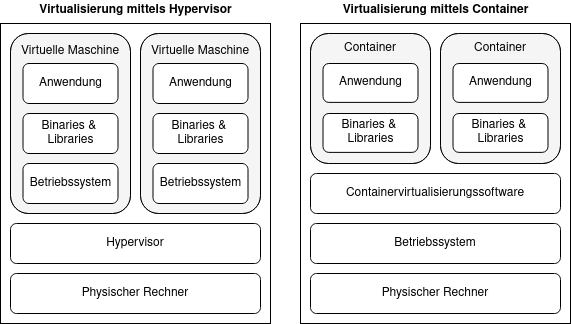
\includegraphics[width=0.95\textwidth]{figures/containervirtualisierung.png}
    \caption{Vergleich Virtualisierung mittels Hypervisor und Container}
\end{figure}

Für die Ausführung einer Anwendung werden Abhängigkeiten wie Bibliotheken, Compiler und Interpreter benötigt. Des Weiteren muss die Anwendung richtig konfiguriert werden. Vor allem bei einer Microservice-Architektur kann das ein Problem werden, da die Microservices über große Netzwerke verteilt auf verschiedenartigen Rechnern bereitgestellt werden sollen. Containervirtualisierung löst dieses Problem, mit einem standardisierten Image-Datei, das die Anwendung mitsamt aller Abhängigkeiten und Konfigurationen beinhaltet [\cite[S. 9]{arundelCloud2019}]. Diese Image-Datei läuft unabhängig von der Plattform auf jedem Rechner, sofern die zugehörige Containervirtualisierungssoftware installiert ist. \\
\\
Eine freie Software zur Containervirtualisierung ist Docker. Es ergänzt die Containervirtualisierung mit benutzerfreundlichen Werkzeugen  und ist der Branchenstandard für Containervirtualisierung. Docker basiert auf der Virtualisierung mit Linux-Containern. Durch herkömmliche Virtualisierung kann Docker jedoch auch auf anderen Betriebssystemen betrieben werden. Im Folgenden werden die wichtigsten Begriffe und Funktionen von Docker näher beschrieben. \\
\\

\subsubsection{Docker Image}

Ein Docker Image ist das Speicherabbild eines Containers. Das Image beinhaltet alle Informationen, die zum Starten eines Containers notwendig sind.  Bei Docker besteht das Image aus mehreren Schichten. Jede Schicht repräsentiert eine Abhängigkeit oder Konfiguration, welche für die Anwendung benötigt wird. Docker optimiert automatisch den verwendeten Speicherplatz durch Wiederverwendung, wenn zwei Images eine gleiche Schicht verwenden. Die Docker Images sind portabel. Über zentrale Registrys können die Images verwaltet, gespeichert und verteilt werden. Docker Hub ist die größte öffentliche Registry mit einer Vielzahl an Images, die von anderen Benutzern bereitgestellt werden. Beim Ausführen eines Images wird auf Basis des Images ein Container gestartet. Das Image ist wiederverwendbar und es können beliebig viele Container aus einem Image erzeugt werden. 

\subsubsection{Dockerfile}

Ein Dockerfile ist eine Textdatei mit mehreren Befehlen, die ein Docker Image beschreiben. Aus einem Dockerfile kann das entsprechende Image gebaut werden. Dazu werden die einzelnen Befehle abgearbeitet und für jeden Befehl eine neue Schicht in dem zugehörigen Image angelegt. Begonnen wird meistens mit einem Basis-Image, welches bereits vorhanden ist. Danach folgen spezifische Änderungen, damit die gewünschte Anwendung ausgeführt werden kann.

\subsubsection{Container}
Ein Container ist die aktive Instanz eines Images. Er besitzt eine begrenzte Lebensdauer und wird, nachdem der in ihm laufende Prozess abgeschlossen ist, beendet. Container sind in der Regel unveränderlich. Soll ein Container geändert werden, so wird der alte Container gegen einen neuen ausgetauscht. Jeder Container besitzt sein eigenes Dateisystem, Anteil an CPU, Speicher und Prozessraum. Er besitzt auch seine eigenen Bibliotheken, Compiler und Interpreter und ist so unabhängig von allen Softwareversionen, die auf dem eigentlichen Betriebssystem installiert sind. Lediglich der Kernel wird geteilt und bildet somit die einzige Abhängigkeit. 

\begin{figure}[H] 
    \centering
    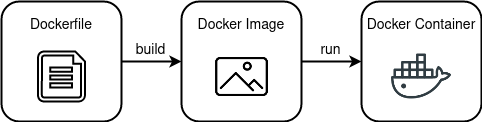
\includegraphics[width=0.8\textwidth]{figures/DockerFileImageContainer.png}
    \caption{Weg vom Dockerfile zum Container}
\end{figure}

\subsection{Kubernetes}

Wenn Microservices in Containern bereitgestellt werden, wird es schnell nicht mehr möglich, die Container manuell bereitzustellen. Auch die Skalierung und die Lastverteilung gestaltet sich als aufwendig. Die Open-Source-Plattform Kubernetes versucht diese Probleme zu lösen. Der Name "Kubernetes" stammt aus dem griechischen und bedeutet soviel wie Steuermann. Kubernetes hilft bei der Koordination und Sequenzierung verschiedener Aktivitäten. Darüber hinaus unterstütze die Plattform bei der Verwaltung der verfügbaren Ressourcen und bei einer effizienten Lastverteilung [\cite[S. 11]{arundelCloud2019}]. Kubernetes bietet somit viele Funktionen, die helfen eine Microservice-Architektur umzusetzen. Häufig wird Kubernetes mit Docker verwendet, es unterstützt aber auch andere Anwendungen zur Containervirtualisierung.

\subsubsection{Aufbau}

Die größte Organisationseinheit der Plattform ist ein Kubernetes Cluster. Ein Cluster besteht aus mindestens einem Control Plane und einem Node. Der Control Plane verwaltet sämtliche Nodes. Um Ausfallsicherheit zu gewährleisten können auch mehrere Control Planes in einem Cluster betrieben werden. Ein Control Plane enthählt eine Key-Value-Datenbank etcd. In ihr wird die gesamte Konfiguration des Clusters gespeichert. Des Weiteren enthält der Control Plane einen \ac{API}-Server, mit der die Nodes kommunizieren. Auch externe Komponenten können mit ac{API}-Server kommunizieren und so Informationen abfragen oder das Cluster konfigurieren. Der Controller Manager steuert über den ac{API}-Server die einzelnen Nodes. Des Weiteren besitzt der Control Plane einen Scheduler, der die Last verteilt und überwacht.  \\
\\
In der Regel besteht ein Cluster aus vielen Nodes. Dabei kann es sich um physische Rechner aber auch um virtuelle Maschinen handeln. Auf den Nodes laufen die Container mit den eigentlichen Anwendungen. Außerdem besitzt jeder Node einen Kubelet. Dieser Kubelet kommuniziert mit dem Controller Manager und verwaltet den Status der Container auf dem jeweiligen Node. \\
\\
{https://kubernetes.io/docs/concepts/overview/components/}

\begin{figure}[H] 
    \centering
    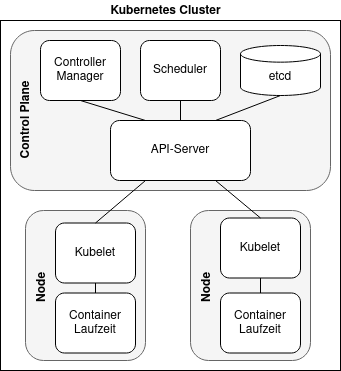
\includegraphics[width=0.75\textwidth]{figures/KubernetesCluster.png}
    \caption{Aufbau eines Kubernetes Cluster}
\end{figure}

\subsubsection{Objekte}

Kubernetes stellt eine Reihe von abstrakten Objekten zur Verfügung, mit denen der Status des Systems dargestellt wird und welche es erleichtern eine Microservice-Architektur zu bauen [\cite[S. 13]{hightowerKubernetes2018}]. Diese Objekte werden in Manifesten beschrieben. Bei den Manifesten handelt es sich um YAML-Dateien. Die Manifeste sind deklarativ aufgebaut, das bedeutet der gewünschte Ausgangszustand wird beschrieben. Nachdem das Manifest übergeben wurde, führt Kubernetes die entsprechenden Aktionen aus, um den beschriebenen Zustand zu erreichen. \\
\\
Pods sind die kleinste einsetzbare Einheit von Kubernetes. Ein Pod repräsentiert eine einen einzelnen Container oder eine Gruppe von Containern. Alle Container in einem Pod laufen immer auf dem gleichen Node. Um eine Menge zusammengehöriger Pods zu verwalten, gibt es Deployments. Deployments repräsentieren eine Anwendung. 

\begin{itemize}
\item Pods sind die kleinste einsetzbare Einheit. Ein Pod besteht aus einem Container oder mehreren zusammengehörigen Containern.
\item: Namespaces werden zur logischen Unterteilung des Clusters verwendet. Sie können zur Isolation verschiedener Entwicklerteams oder Anwendungsmodule genutzt werden.
\item: Services bieten Adressen und Lastverteilung für einen Pod oder mehrere gleichartige Pods.
\item: Volumes bieten persistenten Speicher, der auch nach der Lebenszeit eines Pods bestehen bleibt.
\item: ConfigMaps ermöglichen das Speichern von Konfigurationsdaten als Key-Value-Paare. Sie können beispielsweise von Pods als Umgebungsvariablen konsumiert werden.
\item Deployments repräsentieren eine zustandslose Anwendung beziehungsweise eine Microservice. Durch Deployments kann eine Menge an zusammengehörigen Pods verwaltet und konfiguriert werden. 
\item StatefulSets sind vergleichbar mit Deployments, jedoch für zustandsbezogene Anwendungen.
\item Labels können anderen Objekten zugeordnet werden, um diese zu Gruppieren.
\end{itemize}

Die Kubernetes Objekte werden durch Ressourcen-Manifeste beschrieben. Manifeste
sind deklarativ und üblicherweise im YAML-Dateiformat.

%\subsubsection{Bereitstellung}
%
%-> Deployments
%
%\subsubsection{Service Discovery}
%
%-> Services
%
%\subsubsection{Load Balancing}
%
%-> Service
%
%\subsubsection{Skalierung}
%
%-> Autoscaling

\subsubsection{Kubectl}

Kubectl ist der offizielle Kubernetes-Client und dient der Steuerung von Kubernetes. Bei Kubectl handelt es sich um ein Befehlszeilenwerkzeug für die Interaktion mit dem \ac{API}-Server des Control Planes. Mit kubetl können beispielsweise Objekte verwaltet werden und der Status des gesamten Clusters untersucht werden.

\subsubsection{Minikube}

Minikube ist ein Werkzeug, um ein lokales Kubernetes Cluster zu betreiben. Minikube erstellt ein Cluster bestehend aus nur einem Node in einer virtuellen Maschine. Der Node fungiert dabei sowohl als Control Plane sowie auch als Node. Minikube unterstützt mittlerweile auch den Betrieb mit mehreren Nodes. Des Weiteren kann das gesamte Cluster selbst auch in einem Docker Container anstatt in einer virtuellen Maschine betrieben werden. Minikube erstellt beim Start automatisch eine kubectl-Konfiguration, welche auf das Cluster zeigt und somit über kubectl-Befehle gesteuert werden kann. 